\documentclass[12pt]{article}

\usepackage[utf8]{inputenc}

% dot2tex
\usepackage[x11names, svgnames, rgb]{xcolor}
\usepackage{tikz}
\usetikzlibrary{snakes,arrows,shapes}
\usepackage{amsmath}
\usepackage{standalone}

% doesn't wrap
\usepackage{xcolor}
\definecolor{light-gray}{gray}{0.95}
\newcommand{\code}[1]{\colorbox{light-gray}{\texttt{#1}}}

%\newcommand{\math}[1]{\colorbox{light-gray}{\texttt{#1}}}

\usepackage{times}      % font
\usepackage{graphicx}   % include graphics
\usepackage{fullpage}   % book margins -> std margins
\usepackage{amsmath}    % {align}
%\usepackage{wrapfig}    % {wrapfigure}
%\usepackage{moreverb}   % \verbatimtabinput
%\usepackage{subfig}     % sub-figure
\usepackage{subcaption}
\usepackage[colorlinks]{hyperref}   % pdf links
\usepackage{url}        % url support


% ieee style
\bibliographystyle{ieeetr}

% define "\fig"
\def\fig#1#2{\begin{figure}[!ht]\begin{center}
\includegraphics[width=0.5\textwidth]{#1.jpg}
\end{center}\caption{#2}\label{#1}\end{figure}}

\def\wide#1#2{\begin{figure*}[hptb]\begin{center}
\includegraphics[height=0.5\textwidth]{#1.jpg}
\end{center}\vspace{-0pt}\caption{#2}\label{#1}\end{figure*}}

% create new commands
\def\^#1{\textsuperscript{#1}}
\def\!{\overline}
\def\degree{\ensuremath{^\circ}}

% for hyperref
\hypersetup{
  linkcolor=blue,
  urlcolor=blue,
  filecolor=blue,
  citecolor=blue, % that's it
  pdfauthor={\@author},
  pdftitle={\@title},
  pdfsubject={\@title},
  pdfpagemode=UseNone
}

% info
\author{Neil Edelman}
\title{Prefix-B-trees as an Index}
\date{2021}

\begin{document}

\maketitle

\abstract{This is the abstract.}

\section{Introduction}

\noindent
Intro.\cite{morrison1968patricia}\cite{fredkin1960trie}\cite{knuth1997sorting}

\subsection{Abstract Data Type}

This is a set on a variable-length key, always terminated by a sentinel (allow a string is a prefix of another string in the same trie). It is ordered, and permits range queries with a prefix.

For proper ordering, most-significant bit first; prefix strings the sentinel should be less-than the encoding of all the characters. In practice, a null-terminated string. A Modified~UTF-8 example is Figure~\ref{bits}. It stores the keys in lexicographic order, but not by any collation algorithm.

terminator, like in that paper; a terminator will . This terminator should have less-than all the other characters for ordering, so by a \emph{string} we mean \emph{a null-terminated string}. ; for example, in Modified UTF-8, \code{Z < a < z < æ}. show a picture

\begin{figure} %[!ht]
	\centering
	\subcaptionbox{A cat\label{bits}}{\input{targets/colour-3-add-logic.gv.tex}}
	%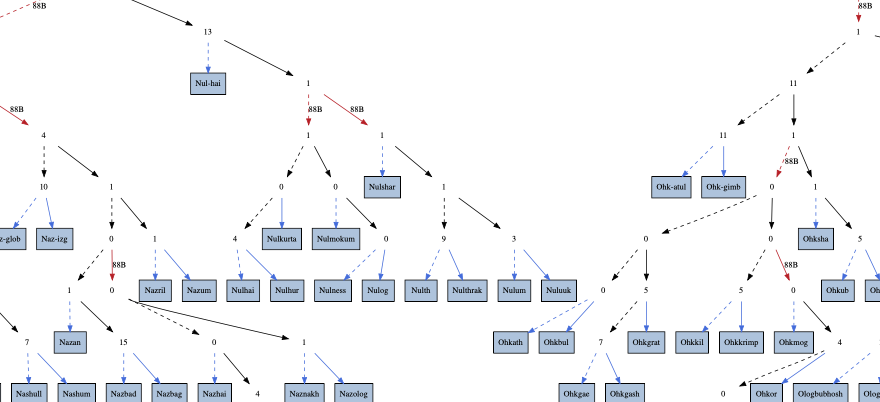
\includegraphics[width=0.5\textwidth]{trie.png}
	\caption{Trie.\label{trie}}
\end{figure}

\subsection{Implementation}

An implementation is an associative-array Patrica trie \cite{}: binary, storing only bit differences; Figure~\ref{prefix:logic}.

This is an index: unlike a binary search where the key is retrieved and compared, we have the string decision bit in the key that cuts down the size of the search space. When we get a prefix match, only one string needs to be retrieved to check that it's a match with all the bits that we skipped over.

\subsection{Tree Structure}

non-empty complete binary tree

semi-implicit: lose the ability to go up the tree; have to have the size \ref{prefix:mem}

\subsection{Machine Considerations}

The data has been engineered for maximum effectiveness of the cache in reading and traversing. That is, the tree structure and the string decisions have been reduced to each a byte and placed at the the top of the data structure of the tree. The size of this sub-structure should be a multiple of the cache line size, while also maximizing the dynamic range allowed for each byte; a trie (also a B-tree) of order 256 is an obvious choice.

instead of adding in one big trie, where the data type presents a limit of how big it is, we have pointers to sub-blocks. This is seen in ... This allows us to shrink the data-type significantly; for a non-empty complete binary tree that has `n` leaves (order `n`), it has `n - 1` the internal nodes, or branches. The maximum that the left branch count can be is when the right node of the root is a leaf, that is `n - 2`. If we set this left-branch maximum to the maximum of the data type, we can use all the range. Practically, we set it to 254 instead of 255; the branches take up 255, and the branch size number is 1, for alignment.

\subsection{Limits}

Worst-case $\{ a, aa, aaa, aaaa, ... \}$. The case where the trie has strings that are bounded, as the tree grows, we can guarantee . . .

This is valid, $\{ dictator \}$, as well as, $\{ dictator, dictionary, dictionaries \}$, but one ca'n't transition to $\{ dictionary, dictionaries \}$: it is too long a skip value. There are several modifications that would allow this, but they are out of this scope.

Insertion: Any leaf on the sub-tree queried will do; in this implementation, favours the left side.

on split, do we have to go locally and see if we can join them?

\bibliography{trie}

\end{document}
